% G07 - Fase 2, Entrega 02 - slides de apoio (10 min: 7 de exposicao + 3 de perguntas)
% xelatex apresentacao.tex
\documentclass[aspectratio=169,10pt]{beamer}
\usetheme{default}
\usepackage{fontspec}
\setsansfont{TeX Gyre Heros}
\usepackage{booktabs,amsmath}
\usepackage{newunicodechar}
\newunicodechar{Ω}{\ensuremath{\Omega}}
\newunicodechar{→}{\ensuremath{\to}}
\newunicodechar{×}{\ensuremath{\times}}
\newunicodechar{·}{\ensuremath{\cdot}}
\definecolor{az}{HTML}{1F5FA8}\definecolor{vm}{HTML}{C0392B}
\setbeamercolor{frametitle}{fg=az}\setbeamercolor{structure}{fg=az}
\setbeamertemplate{navigation symbols}{}
\setbeamertemplate{footline}{\hfill\scriptsize\color{gray}G07 · ECOM060 · E02 \quad\insertframenumber\hspace{1em}\vspace{4pt}}
\newcommand{\fig}[2][\textwidth]{\includegraphics[width=#1]{../relatorio/figuras/#2}}
\begin{document}

\begin{frame}
\vspace{1.2cm}
{\small\color{vm} Grupo G07 · ECOM060 Instrumentação Eletrônica · UFAL 2026.2 · Fase 2, Entrega 02}\\[6pt]
{\LARGE\bfseries\color{az} Equivalente elétrico no TyphoonSim:\\ motor BLDC MOONS' R42BLD30L3}\\[10pt]
Nícolas De Almeida Souza · Lucas Momesso Alves · Cláudio Henrique da Costa Santos
\begin{columns}\column{.55\textwidth}
\vspace{6pt}\small
\begin{itemize}
\item Pendências da E01: imagem do sistema completo (não há motor físico) e método de simulação detalhado (Tab.~1 do relatório).
\item O bloco \texttt{Brushless DC Machine} sai; no lugar entra um circuito de R, L e fontes controladas.
\end{itemize}
\column{.4\textwidth}\centering
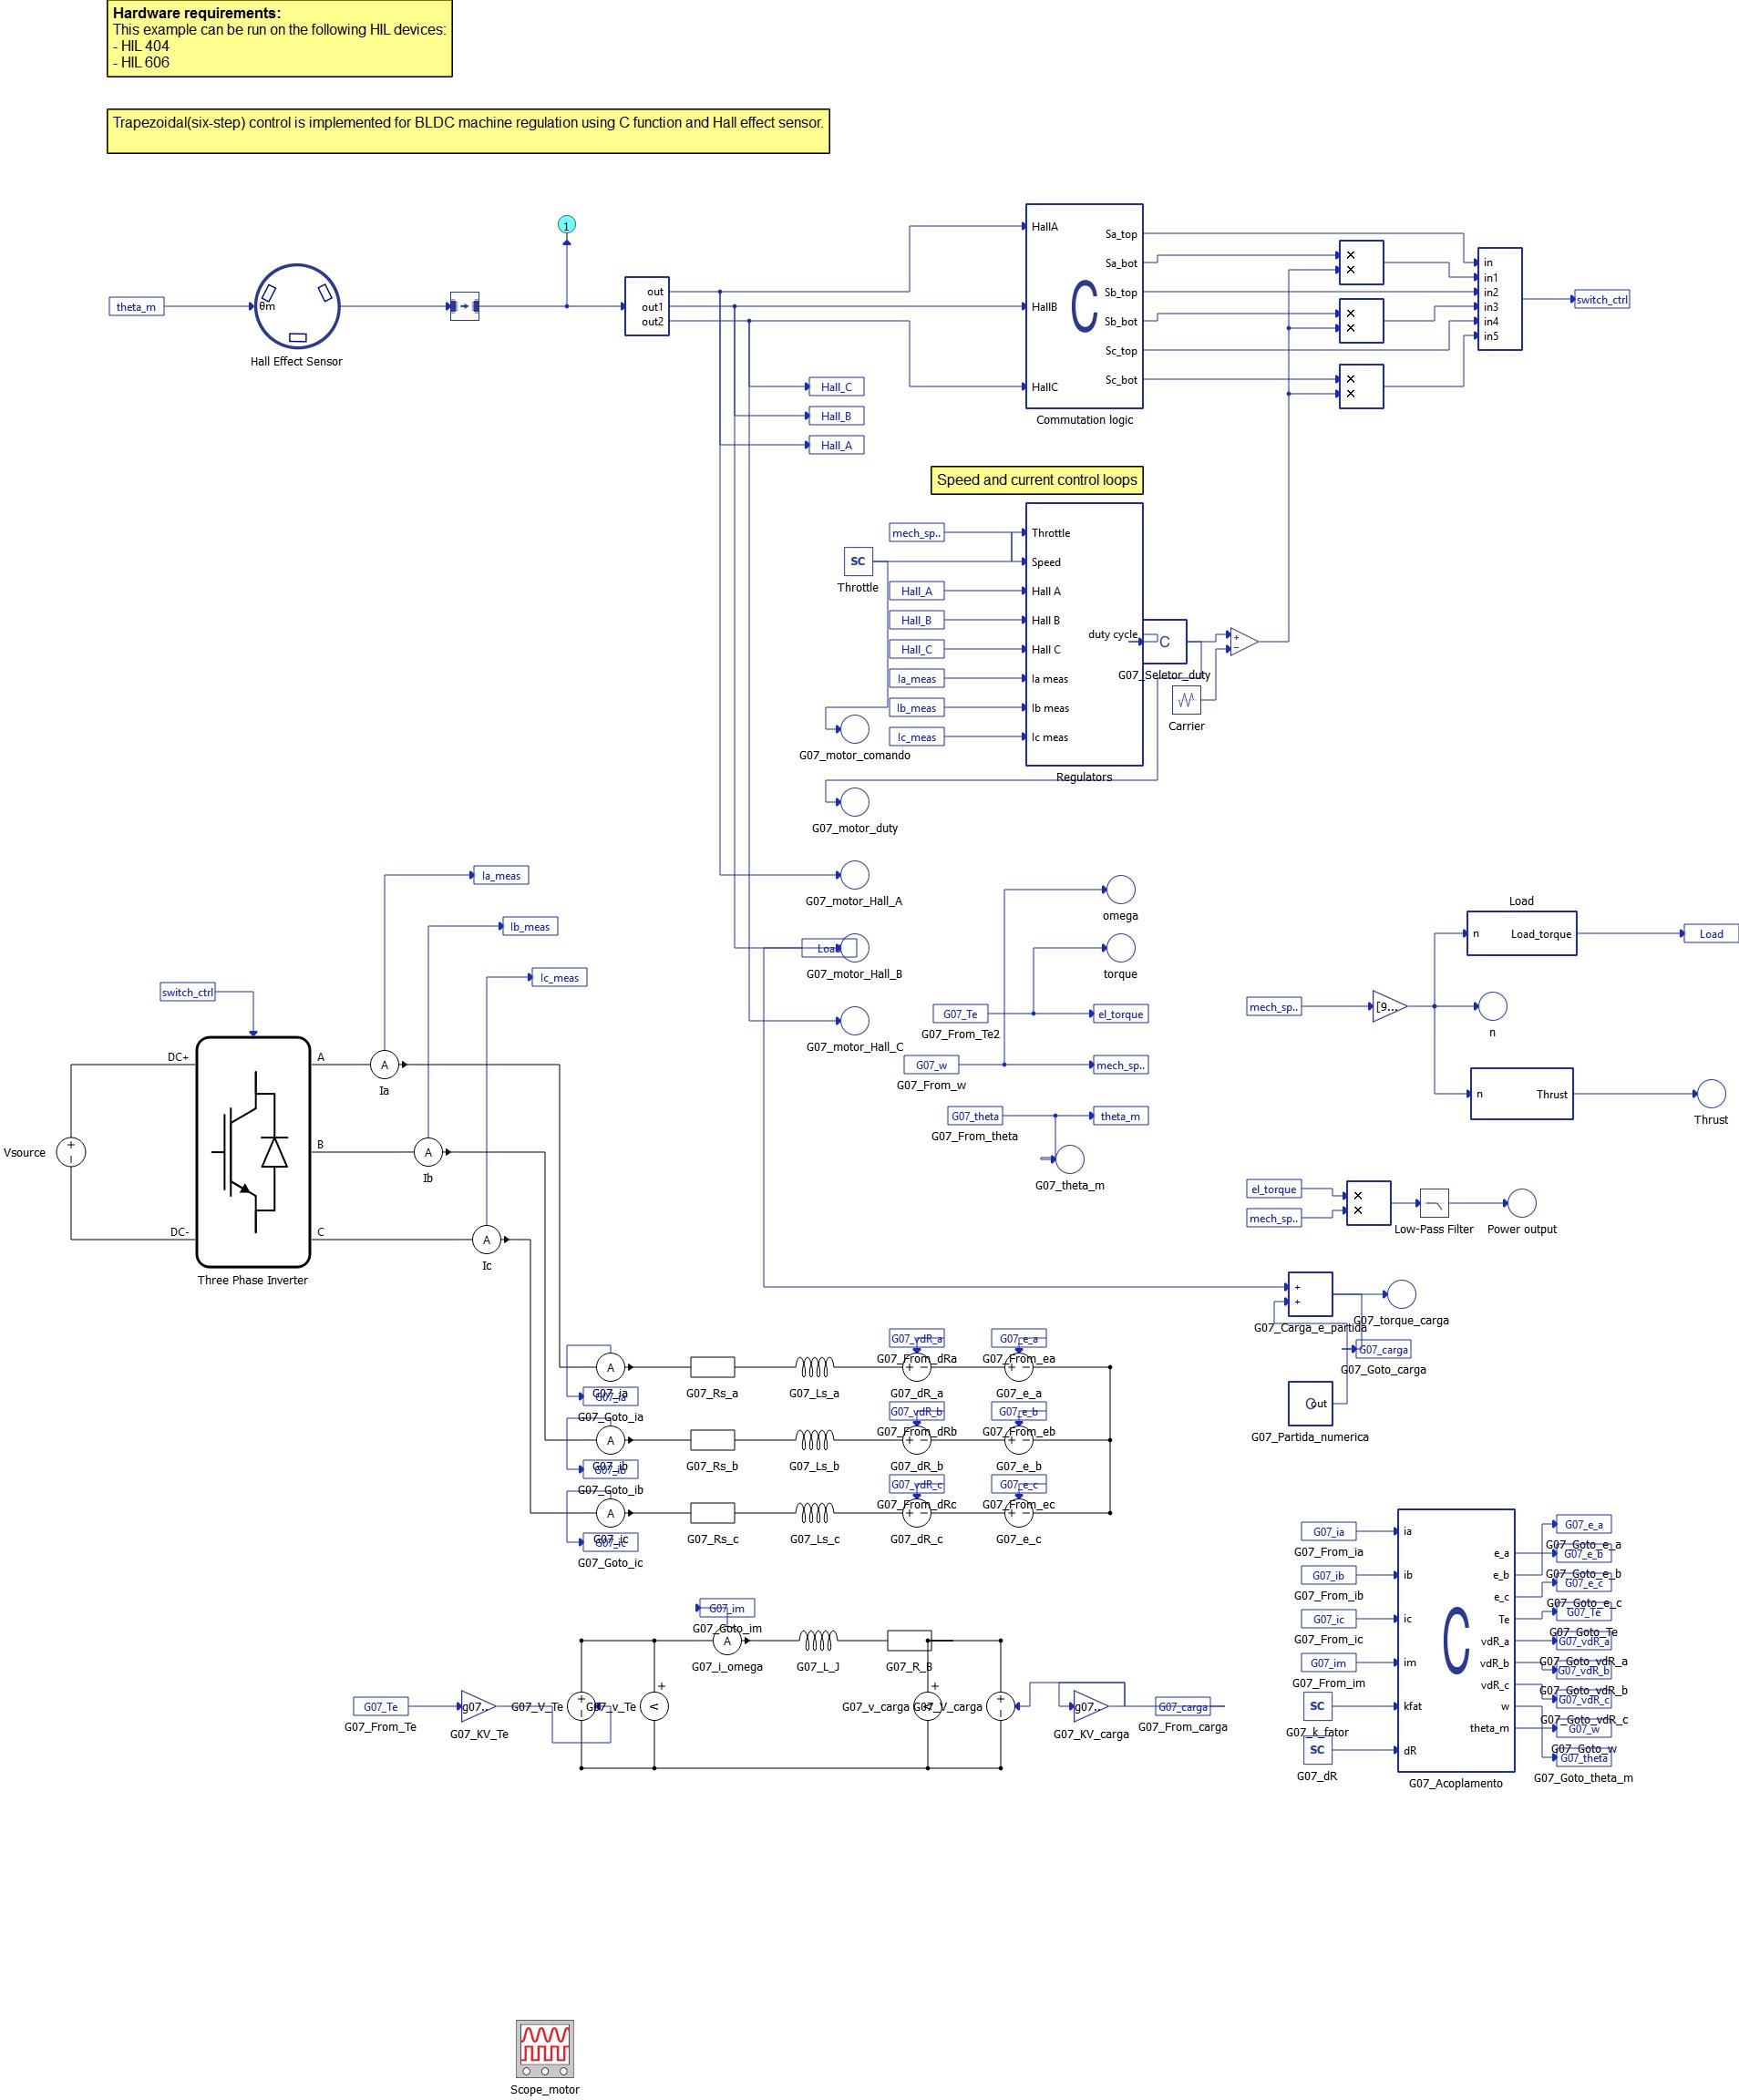
\includegraphics[height=3.2cm]{../relatorio/figuras/foto_motor.jpg}
\end{columns}
\end{frame}

\begin{frame}{Analogia força–tensão (2 min)}
\begin{columns}[T]\column{.5\textwidth}\small
\begin{tabular}{ll}\toprule original & circuito\\\midrule
torque (esforço) & tensão, $K_V$ = 100 V/(N·m)\\
velocidade (fluxo) & corrente, 1 A = 1000 rpm\\
inércia $J$ & indutor $L_J$ = 34,56 mH\\
atrito $B$ & resistor $R_B$ = 10,47 mΩ\\
$T_e$, carga, $T_d$ & fontes de tensão controladas\\
FCEM $e_x$ & fonte controlada por $i_m$\\
$R_s$, $L_s$, $V_s$, inversor & 1:1\\\bottomrule\end{tabular}
\column{.48\textwidth}\small
$L_J\dot i_m+R_Bi_m=v_{Te}-v_{carga}$\\
$\Leftrightarrow\;J\dot\omega+B\omega=T_e-T_L-T_d$\\[4pt]
\begin{itemize}
\item Escala de tempo 1:1, em tempo real no HIL.
\item $k/K_I$ = 5,027 V/A, o mesmo valor do \texttt{Emf} da E01.
\item Polos, $\omega_n$, $\zeta$, $\tau_m$ e ganho estático idênticos à R2 da E01:\\ $-479{,}1\pm j227{,}9$ s$^{-1}$ em 4000 rpm.
\end{itemize}
\end{columns}
\end{frame}

\begin{frame}{Circuito no TyphoonSim e inventário (2 min)}
\centering\fig[.82\textwidth]{fig_circuito.pdf}\\[-2pt]
\scriptsize Nativos: \texttt{Resistor}, \texttt{Inductor}, \texttt{Signal Controlled Voltage Source}, \texttt{Current/Voltage Measurement}, \texttt{Gain}, \texttt{SCADA Input}. \textbf{Uma} \texttt{C function} (25 linhas): trapézio $f(\theta_e)$, produtos $\omega f$ e $\sum f i$, $\theta_m$ envolto em $2\pi$. A biblioteca não tem FCEM trapezoidal nem girador fora do bloco BLDC.
\end{frame}

\begin{frame}{Modelo completo no Schematic Editor}
\centering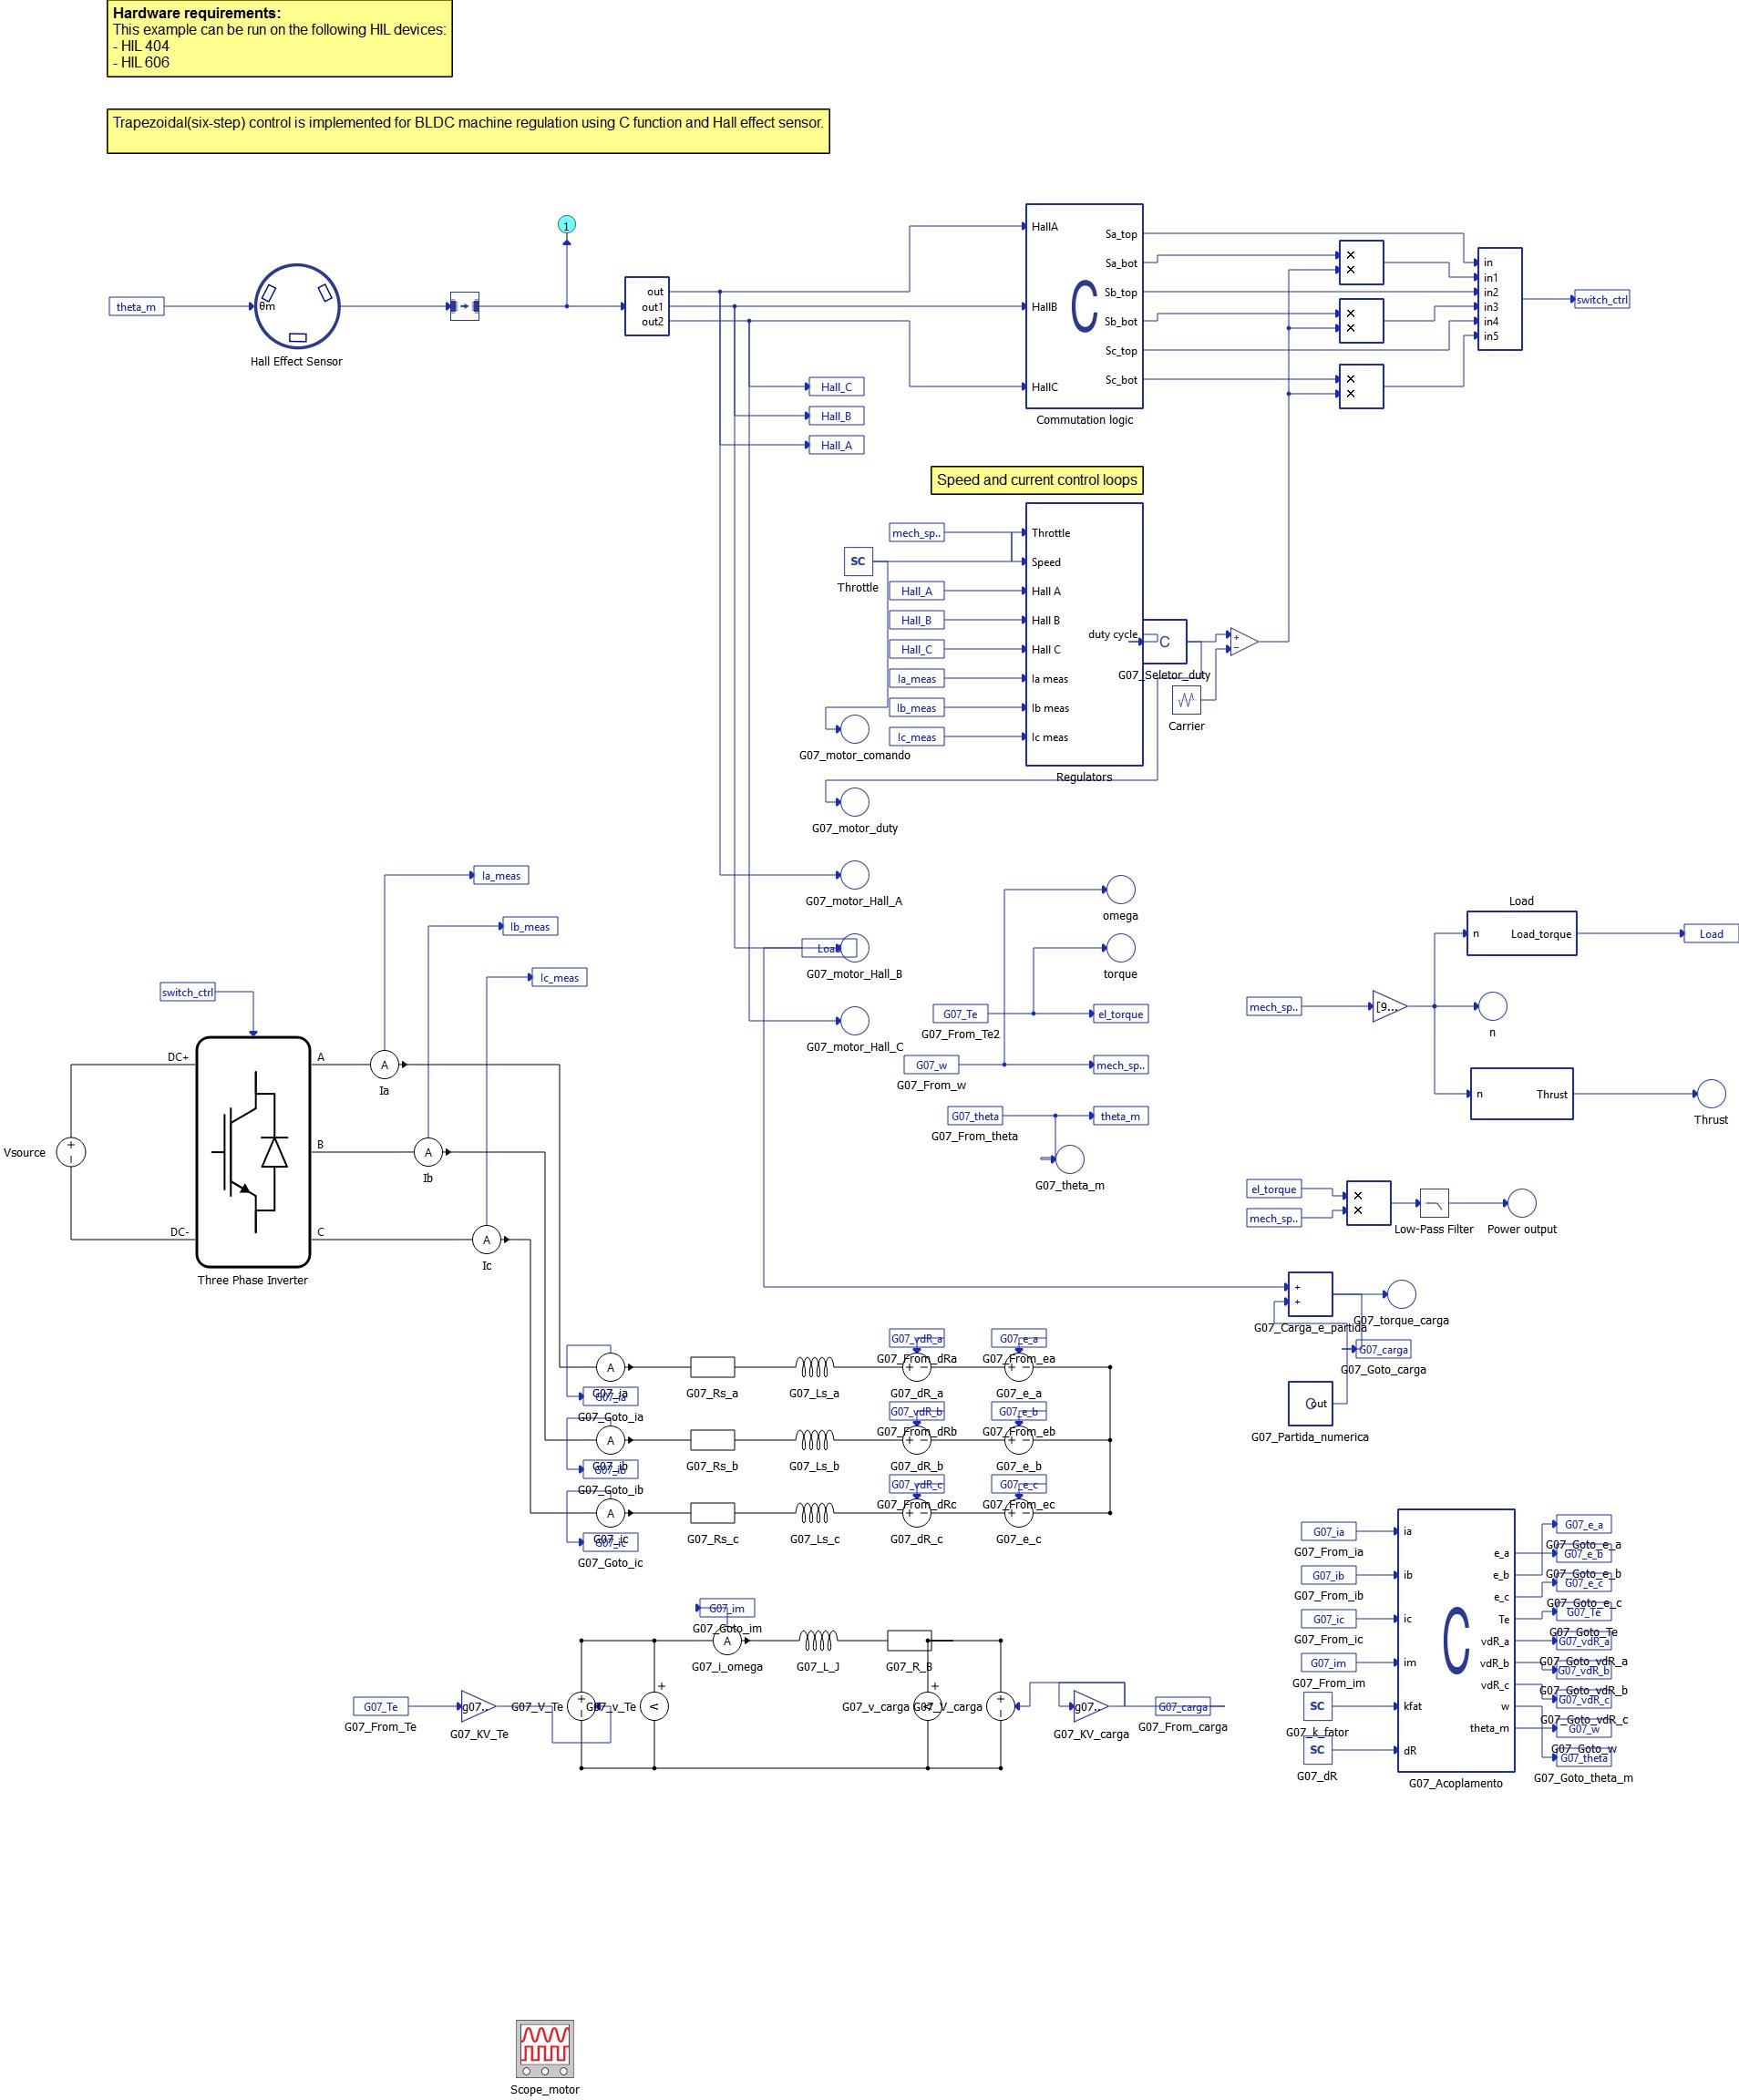
\includegraphics[height=.84\textheight]{../relatorio/figuras/foto_motor.jpg}
\end{frame}

\begin{frame}{Validação no VHIL/SCADA × E01 (2 min)}
\centering\fig[.74\textwidth]{fig_validacao.pdf}\\
\scriptsize 6 ensaios compilados para o Virtual HIL e gravados pelo \emph{Capture} do HIL SCADA (0,3 s, 50 kS/s). Critério: regime $\le$ 0,5 \%; tempos $\le$ 5 \% (grandes sinais), $\le$ 10 \% (degrau pequeno). \textbf{19 de 22 itens passam}.
\end{frame}

\begin{frame}{Fora do equilíbrio e diferenças}
\begin{columns}\column{.55\textwidth}\fig{fig_correntes.pdf}
\column{.43\textwidth}\scriptsize
\begin{itemize}
\item Desaceleração livre (Riccati): $\le$ 0,17 \%; $t_{1/2}$ +0,01 \%. Malha fechada e pulso MF: $\le$ 0,07 \%. Pulso MA: $\Delta n$ $-$0,8 \%.
\item Condução descontínua ($d$ = 0,55): termina em 0,52 ms contra 0,51 ms.
\item PWM em tempo real aplica $d_{ef}$ = 0,759 (TyphoonSim: 0,75): identificado pelo $n_{ss}$ e usado na E01.
\item Fora: $t_{63}$/$t_s$ da partida ($-$7 a $-$8 \%) e ganho do degrau pequeno (+2,9 \%): vêm do modulador; o mesmo \texttt{.tse} no TyphoonSim dá +0,07 \% e +1,4 \%.
\end{itemize}
\end{columns}
\end{frame}

\begin{frame}{Sensibilidade no SCADA (1 min)}
\begin{columns}[T]
\column{.52\textwidth}\centering\fig{fig_sensibilidade.pdf}\\[-2pt]
{\tiny TyphoonSim: $n_{ss}$ a $\le$ 0,4 \% do trifásico da E01; tendência a $\le$ 1,6 \% da Tab.~5.}
\column{.46\textwidth}\scriptsize
\textbf{Executado no VHIL/SCADA} (painel, modelo rodando):\\[3pt]
\begin{tabular}{@{}lccc@{}}\toprule
Ajuste & $n_{ss}$ & razão & E01\\\midrule
nominal & 3458 & 1,000 & 1,000\\
$k\times$0,896 & 3570 & 1,032 & 1,024\\
$k\times$1,3375 & 3068 & 0,887 & 0,891\\
$\Delta R=-1{,}1$ & 3700 & 1,070 & 1,077\\
$\Delta R=+0{,}63$ & 3319 & 0,960 & 0,960\\\bottomrule
\end{tabular}\\[4pt]
Diferença $\le$ 0,8 \%. \textbf{O equivalente responde aos parâmetros como o original}; $J$ só muda recompilando ($L_J$).
\end{columns}
\end{frame}

\begin{frame}{Demonstração e repetibilidade}
\small
\begin{enumerate}
\item Abrir \texttt{modelo\_equivalente.tse} (Typhoon 2026.3, perspectiva TyphoonSim para os ensaios, tempo real para o SCADA) e escolher \texttt{g07\_modo} em \emph{Model initialization}.
\item Compilar para o Virtual HIL e carregar \texttt{painel\_equivalente.cus} no HIL SCADA.
\item Ao vivo: $n\approx$ 3458 rpm; \texttt{G07\_k\_fator} = 1,3375 → $\approx$ 3068 rpm; \texttt{G07\_dR} = $-1{,}1$ Ω → $\approx$ 3700 rpm.
\item Tudo está em um único arquivo: \texttt{modelo\_equivalente.tse}.
\end{enumerate}
\vspace{4pt}
\textbf{Próxima entrega:} a instrumentação mede $i_m$ (velocidade), $v_{Te}$ (torque) e as correntes de fase nesta planta.
\end{frame}
\end{document}
